% Fig. 1: architecture of final-A (full text width). Thumbnails: paper/make_thumbnails.py.
\begin{figure*}[t]
\centering
\begin{tikzpicture}[x=0.975cm, y=0.92cm,
  arch/.style={draw=black!65, rounded corners=1pt, align=center, inner sep=1.1pt,
               font=\fontsize{5.5}{6.3}\selectfont},
  ctx/.style={arch, fill=blue!9}, det/.style={arch, fill=orange!13}, dec/.style={arch, fill=green!10},
  res/.style={arch, fill=gray!12}, train/.style={arch, dashed, fill=red!5},
  lab/.style={font=\fontsize{5.3}{6.1}\selectfont, align=center, inner sep=0.5pt},
  flow/.style={-{Stealth[length=1.1mm, width=0.9mm]}, draw=black!70, line width=0.45pt},
  line/.style={draw=black!70, line width=0.45pt}]
% ---------------- input
\node[inner sep=0] (img) at (0.88,3.2) {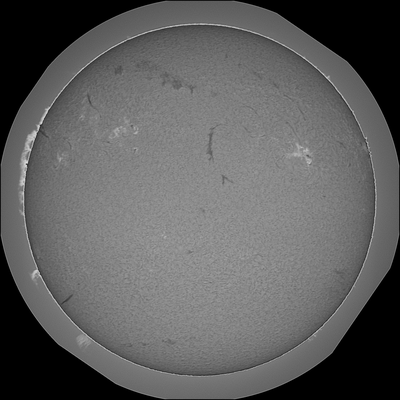
\includegraphics[width=1.66cm]{figures/arch_input.png}};
\node[lab, below=0.5mm of img] {H$\alpha$ image\\2048\textsuperscript{2} px (the\\only inference input)};
\coordinate (split) at (1.98,3.2);
\draw[line] (img.east) -- (split);
% ---------------- context branch
\node[lab, anchor=west] at (2.2,6.16) {\textbf{context branch}: FlashInternImage-L (DCNv4, 219\,M, ImageNet-22k$\to$1k);
  strides relative to 2048\,px};
\node[ctx, text width=0.8cm, minimum height=0.8cm] (rs) at (2.72,5.1) {resize to\\1024\textsuperscript{2}};
\node[ctx, text width=0.82cm, minimum height=1.45cm] (s1) at (3.86,5.1) {S1\\5 blocks\\160 ch\\/8};
\node[ctx, text width=0.82cm, minimum height=1.28cm] (s2) at (4.92,5.1) {S2\\5 blocks\\320 ch\\/16};
\node[ctx, text width=1.0cm, minimum height=1.11cm] (s3) at (6.08,5.1) {S3\\22 blocks\\640 ch\\/32};
\node[ctx, text width=0.82cm, minimum height=0.94cm] (s4) at (7.24,5.1) {S4\\5 blocks\\1280 ch\\/64};
\node[ctx, text width=0.82cm, minimum height=1.45cm] (fpn) at (8.36,5.1) {FPN\\$P_1$--$P_4$\\192 ch\\/8 to /64};
\draw[flow] (split) |- (rs.west);
\foreach \a/\b in {rs/s1, s1/s2, s2/s3, s3/s4, s4/fpn} \draw[flow] (\a) -- (\b);
% ---------------- native detail branch
\node[lab] at (3.7,2.42) {\textbf{native branch}, 2048\textsuperscript{2} px};
\node[inner sep=0] (c1) at (2.72,1.62) {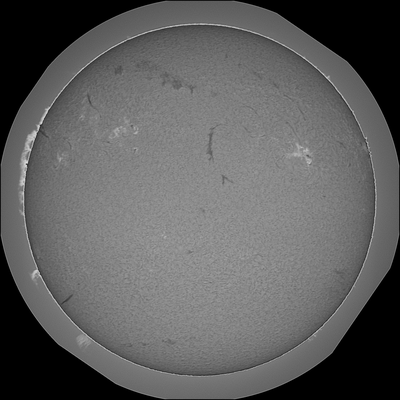
\includegraphics[width=0.84cm]{figures/arch_input.png}};
\node[inner sep=0] (c2) at (3.7,1.62) {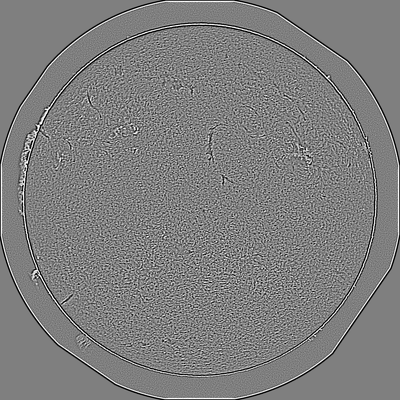
\includegraphics[width=0.84cm]{figures/arch_contrast.png}};
\node[inner sep=0] (c3) at (4.68,1.62) {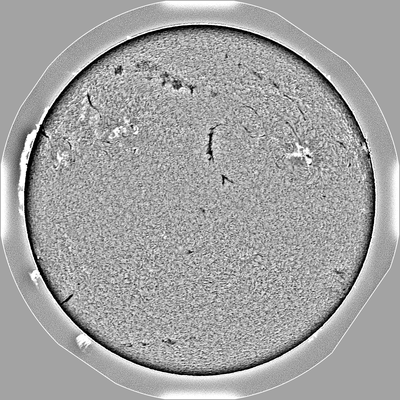
\includegraphics[width=0.84cm]{figures/arch_darkness.png}};
\node[lab, below=0.4mm of c1] {intensity\\$I$};
\node[lab, below=0.4mm of c2] {local\\contrast};
\node[lab, below=0.4mm of c3] {darkness\\$I/B-1$};
\draw[flow] (split) |- (c1.west);
\node[det, text width=0.95cm, minimum height=1.15cm] (h1) at (5.88,1.62) {Haar 2$\times$2\\(4 phases)\\1$\times$1 conv\\32 ch, /2};
\node[det, text width=1.1cm, minimum height=1.15cm] (g2) at (7.05,1.62) {gate $\oplus P_1$\\curve block\\32 ch, /2};
\node[det, text width=1.1cm, minimum height=1.15cm] (g4) at (8.3,1.62) {Haar\\gate $\oplus P_1$\\curve block\\64 ch, /4};
\draw[flow] (c3.east) -- (h1.west);
\draw[flow] (h1) -- (g2);
\draw[flow] (g2) -- (g4);
\draw[line] (fpn.south) -- ++(0,-1.15) coordinate (pdown);
\draw[flow] (pdown) -| (g2.north);
\draw[flow] (pdown) -| (g4.north);
\node[lab, anchor=west] at (8.4,3.4) {$P_1$};
\node[lab, text=black!65] at (7.0,0.72) {\itshape at inference in 512\,px tiles with a 48\,px halo};
\node[det, text width=1.22cm, minimum height=0.46cm] (f4) at (9.76,2.22) {$F_4$: 192 ch, /4};
\node[det, text width=1.22cm, minimum height=0.46cm] (m2) at (9.76,1.62) {$M_2$: 64 ch, /2};
\node[det, text width=1.22cm, minimum height=0.46cm] (ph) at (9.76,1.02) {$\Phi_2$: 32 ch, /2};
\draw[flow] (g4.east) -- (f4.west);
\draw[flow] (g4.east) -- (m2.west);
\draw[flow] (m2) -- (ph);
% ---------------- query decoder
\node[dec, text width=3.5cm, minimum height=0.86cm] (mem) at (12.62,5.1)
  {\textbf{scene memory}: $F_4$, $P_2$, $P_3$ average-pooled to 48\textsuperscript{2}, 24\textsuperscript{2},
   12\textsuperscript{2} cells, plus 256 unpooled $F_4$ tokens at seed-map peaks};
\node[dec, text width=1.0cm, minimum height=0.62cm] (seed) at (11.48,3.82) {seed map\\(skeleton)};
\node[dec, text width=1.0cm, minimum height=0.85cm] (qi) at (11.48,2.92) {64 queries\\at diverse\\seed peaks};
\node[dec, text width=1.9cm, minimum height=2.9cm, align=left] (layer) at (13.36,3.0)
  {\textbf{6 decoder layers}\\[1.2pt]
   $\cdot$ self-attention\\
   $\cdot$ cross-attention to the memory, masked by the query's own mask (global every 2nd layer)\\
   $\cdot$ attention to 64 native points of its mask (32 foreground, 32 edge)\\
   $\cdot$ FFN, mask feedback};
\node[train, text width=2.05cm, minimum height=0.5cm] (pilot) at (13.36,0.8) {+32 mask pilots from noised GT masks (training only)};
\draw[flow] (fpn.east) -- node[lab, above] {$P_2,P_3$} (mem.west);
\draw[line] (f4.east) -- ++(0.24,0) coordinate (bus);
\draw[flow] (bus) |- ([yshift=-2.6mm]mem.west);
\draw[flow] (bus |- seed.west) -- (seed.west);
\draw[flow] (bus) |- ([yshift=-11mm]layer.west) node[lab, above, pos=0.78] {native points};
\draw[flow] (seed) -- (qi);
\draw[flow] (qi.east) -- (qi.east -| layer.west);
\draw[flow] (layer.north |- mem.south) -- (layer.north);
\draw[flow, dashed] (pilot) -- (layer);
% ---------------- heads, native rendering, test-time augmentation
\node[res, text width=1.25cm, minimum height=1.45cm] (head) at (15.22,4.32)
  {per query\\$P(\text{filament})$\\quality $\approx$ IoU\\$e\in\mathbb{R}^{64}$\\$\varphi\in\mathbb{R}^{8}$};
\node[res, text width=1.32cm, minimum height=1.55cm] (rend) at (15.22,2.3)
  {native logits\\$\uparrow_2(e^{\top}\!M_2)$\\$+\,\mathrm{PS}(\varphi^{\top}\Phi_2)$\\$\to$ 2048\textsuperscript{2} px};
\draw[flow] (layer.east |- head.west) -- (head.west);
\draw[flow] (head) -- (rend);
\draw[line] (m2.east) -- ++(0.12,0) coordinate (mbus);
\draw[line] (mbus) -- (mbus |- 0,0.3) coordinate (low);
\draw[line] (ph.south) -- (ph.south |- low);
\draw[flow] (ph.south |- low) -| (rend.south);
\node[res, text width=1.52cm, minimum height=1.5cm] (tta) at (17.1,4.55)
  {$\times$8 dihedral views\\cluster (IoU$>$0.5),\\average; keep\\score $\ge$ 0.10,\\mask $p\ge$ 0.40;\\pixel ownership};
\node[inner sep=0] (out) at (17.1,2.26) {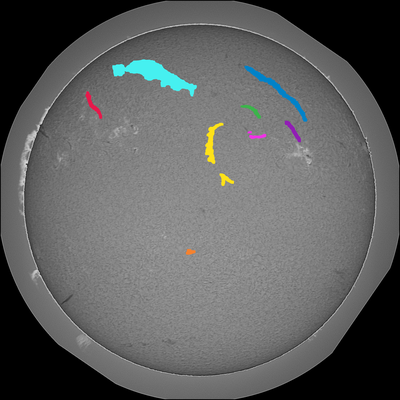
\includegraphics[width=1.55cm]{figures/arch_output.png}};
\node[lab, below=0.5mm of out] {non-overlapping\\instances};
\draw[flow] (rend.east) -- ++(0.22,0) |- (tta.west);
\draw[flow] (tta) -- (out);
% ---------------- training objective
\node[train, text width=5.7cm] (loss) at (14.98,6.12)
  {\textbf{training}: Hungarian matching per annotator record, $-\log\widetilde{\mathrm{PQ}}$ on 16,384 native
   points, auxiliary losses $\times$0.02};
\end{tikzpicture}
\Description{Block diagram: an H-alpha image feeds a context branch (resize, FlashInternImage-L stages, FPN) and a native
branch (intensity, local contrast and darkness channels, Haar split, gated curve blocks); both feed a query decoder whose
per-query heads render native-resolution masks, fused over eight dihedral views into non-overlapping instances.}
\caption{Architecture of final-A (223.6\,M parameters, 97.9\,\% in the backbone) at inference on a test
observation. A pretrained backbone sees the whole disk at 1024\,px, and a native branch reads three physical
channels at 2048\,px. Queries start at peaks of a skeleton-like seed map and render full-resolution masks from a
stride-2 basis $M_2$ plus a pixel-shuffled ($\mathrm{PS}$) phase term. Dashed boxes are training-only.}
\label{fig:pipeline}
\end{figure*}
